\chapter{Use Case}

\begin{figure}
	\begin{center}
		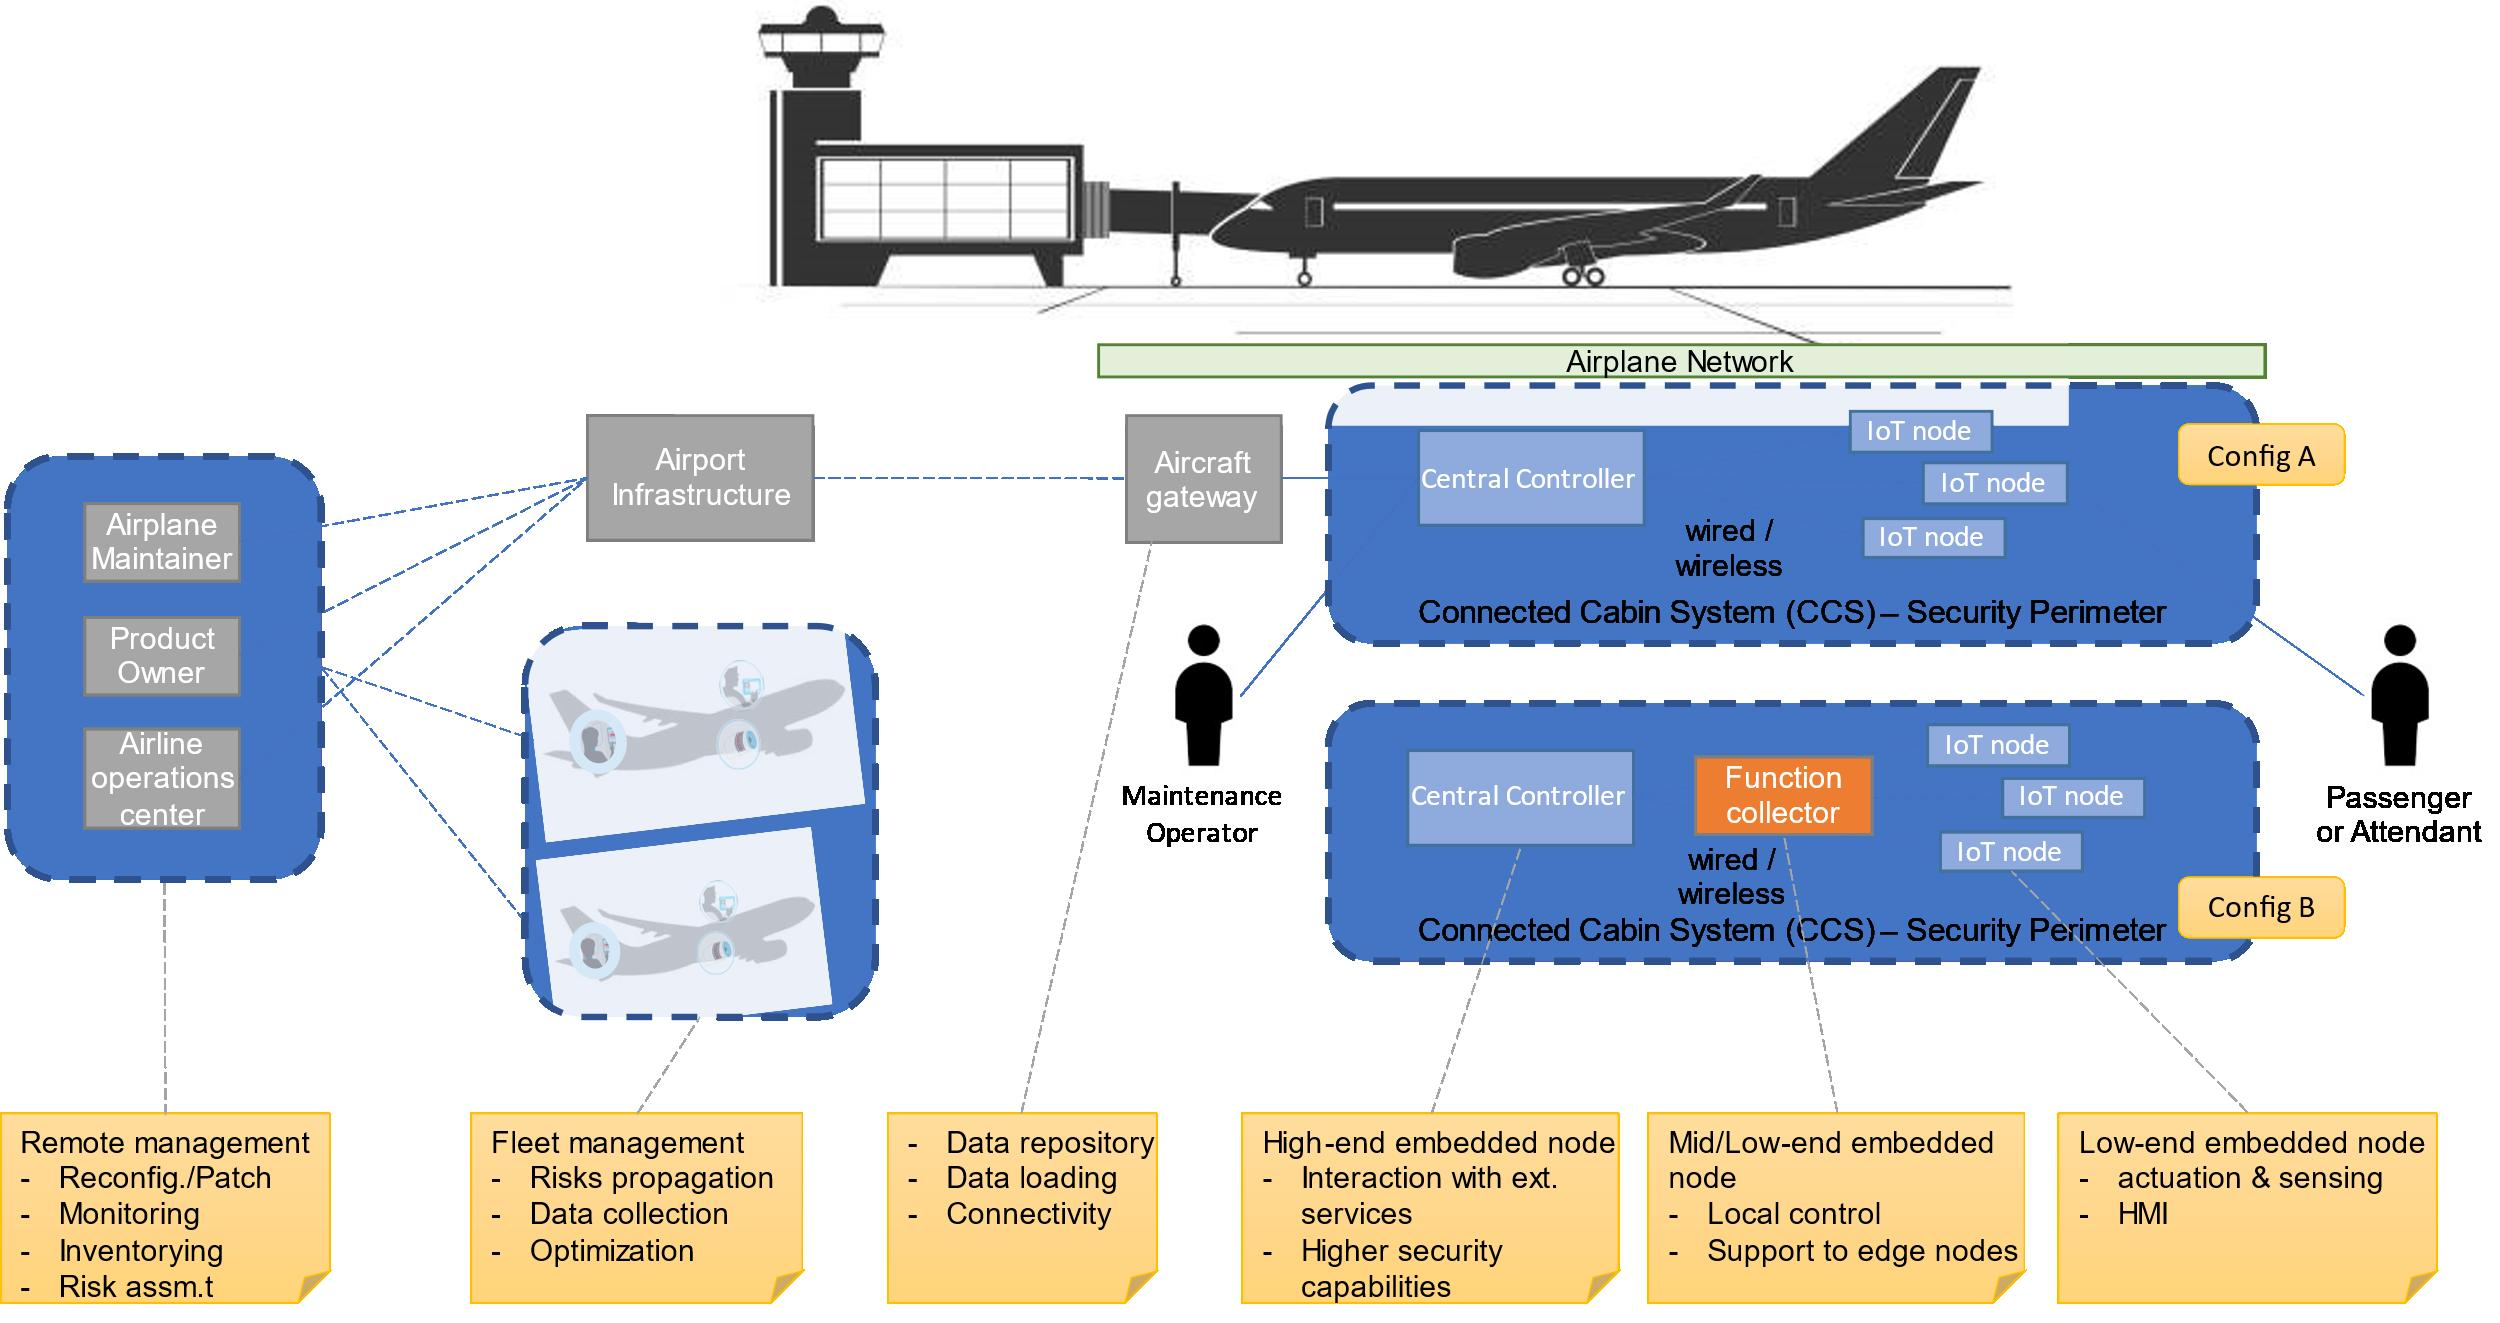
\includegraphics[width=0.95\textwidth]{figures/collins-ccs.jpg}
	\end{center}
	\caption{Collins CCS}
	\label{fig:Collins CCS}
\end{figure}

\section{Background}

Our use case will take the CCS scenario from Figure~\ref{fig:Collins CCS} into consideration and build up on their use cases.

Nowadays more and more IoT devices are being deployed to aircraft cabins to improve passenger experience and airline
operations. Benefits span from remote PHM to reduced maintenance time, while also supporting a
continuous (re)certification process. % TODO: (aver) add source, maybe from certify

\section{Actors}

We will consider following actors for our use case.

\begin{itemize}
	\item Airline:
	      Owns the aircraft and oversees interactions and system operations.
	\item Airplane maintainer: They could be e.g., Airplane manufacturer. Oversees maintenance of the aircraft,
	      including the integration of systems designed by different manufacturers and their configuration.
	\item Product Owner: Oversees design and maintenance of systems deployed in the aircraft on assignment of the
	      airplane maintainer.
	\item Maintenance operator: They work for the airplane maintainer. Their responsibilities include e.g.,
	      the replacement of devices or on-site software upgrades of e.g., portable data loaders.
	\item Passenger, Attendant, Pilot: They interact with the aircraft through sensors, actuators or HMI.
\end{itemize}

\section{System Components}

We will consider an aircraft to have multiple networks, covering various aspects.
\begin{itemize}
	\item In-flight entertainment system
	\item Aircraft System
	\item Flight Maintenance
\end{itemize}

For our use case we will assume config 'A' as the main configuration of the networks, where edge nodes are connected to
a central controller that manages the edge nodes as a subnet.
\begin{itemize}
	\item IoT / Edge Nodes: low-end devices, including actuation, sensing or HMI capabilities, with limited
	      room for hardware and software based cybersecurity, that requires offloading to a more capable
	      instance.
	\item Central Controller: High-end devices with ability to host full-fledged security functionalities.
\end{itemize}

External communication will take place through aircraft gateway offering services for data repository, data loading and
connectivity with external environment. The airline operations center, product owner and airplane maintainer can interact
through the airport infrastructure. A technician may directly access the aircraft if necessary.


\section{Scenarios}
\subsection{Installation of Connected Cabin Systems} % (fold)
\label{sub:Installation of Connected Cabin Systems}

\subsubsection{Goals}

The goals of this scenario include bootstrapping and customization of devices for specific deployment, updating and
decommissioning of previous systems, guaranteeing a reset to a known and fresh, wiped data, state.
Table~\ref{tab:Actors involved} highlights the involved actors and Table~\ref{tab:Lifecycle stages involved} shows the
stages involved in this scenario.

\begin{table}
	\caption{Actors involved}
	\label{tab:Actors involved}
	\begin{center}
		\begin{tabular}{ |p{2.5cm}|p{2.5cm}|p{2.5cm}|p{2.5cm}|p{2.5cm}| }
			\hline
			Airline & Airplane Maintainer & Product Owner & Maintenance Operator & Passenger, Attendant, Pilot \\
			\hline
			X       & -                   & X             & -                    & X                           \\
			\hline
		\end{tabular}
	\end{center}
\end{table}

\begin{table}
	\caption{Lifecycle stages involved}
	\label{tab:Lifecycle stages involved}
	\begin{center}
		\begin{tabular}{ |c|c|c|c|c| }
			\hline
			Bootstrapping & Operation & Update & Repurposing & Decommissioning \\
			\hline
			X             & -         & X      & -           & X               \\
			\hline
		\end{tabular}
	\end{center}
\end{table}


% TODO: (aver) continue copying over markdown

% subsection Installation of Connected Cabin Systems (end)
